\chapter[Подготовка КД]{Подготовка конструкторской документации в Altium Draftsman}

\section{Приготовления}

Для начала приведём в порядок параметры компонентов:
\begin{itemize}
	\item Компоненты с одинаковым номиналом и посадочным местом должны группироваться
	\item Параметр Package должен соответствовать реальному типоразмеру
	\item У компонентов должны быть заполнены поля с информацией о режимах работы
\end{itemize}
\begin{figure}[H]
	\centering
	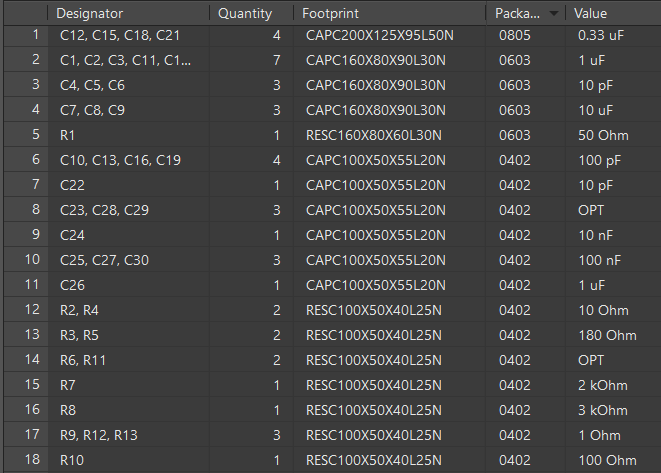
\includegraphics[width=0.8\textwidth]{DiscreteDocBom.png}
	\caption{Порядочная таблица.пнг}%
	\label{fig:DiscreteDocBom}
\end{figure}

Импортируем шаблоны из библиотеки \href{https://github.com/dee3mon/altium-templates}{altium-templates} и приступим к экспортированию КД средствами Altium Draftsman + GOSTBOM.

Децимальные номера будут выбираться исходя из определения --- всё , что относится к изделию имеет номер 464342, а всё, что к печатной плате --- 687254.

\section[Создание сборочного чертежа на печатный узел]{Создание сборочного чертежа на печатный узел (МПСУ.464342.21-005СБ)}

Выберем шаблон A3. На первый лист добавим главный вид и вид сбоку, настроим отображение, проставим размеры.
\begin{figure}[H]
	\centering
	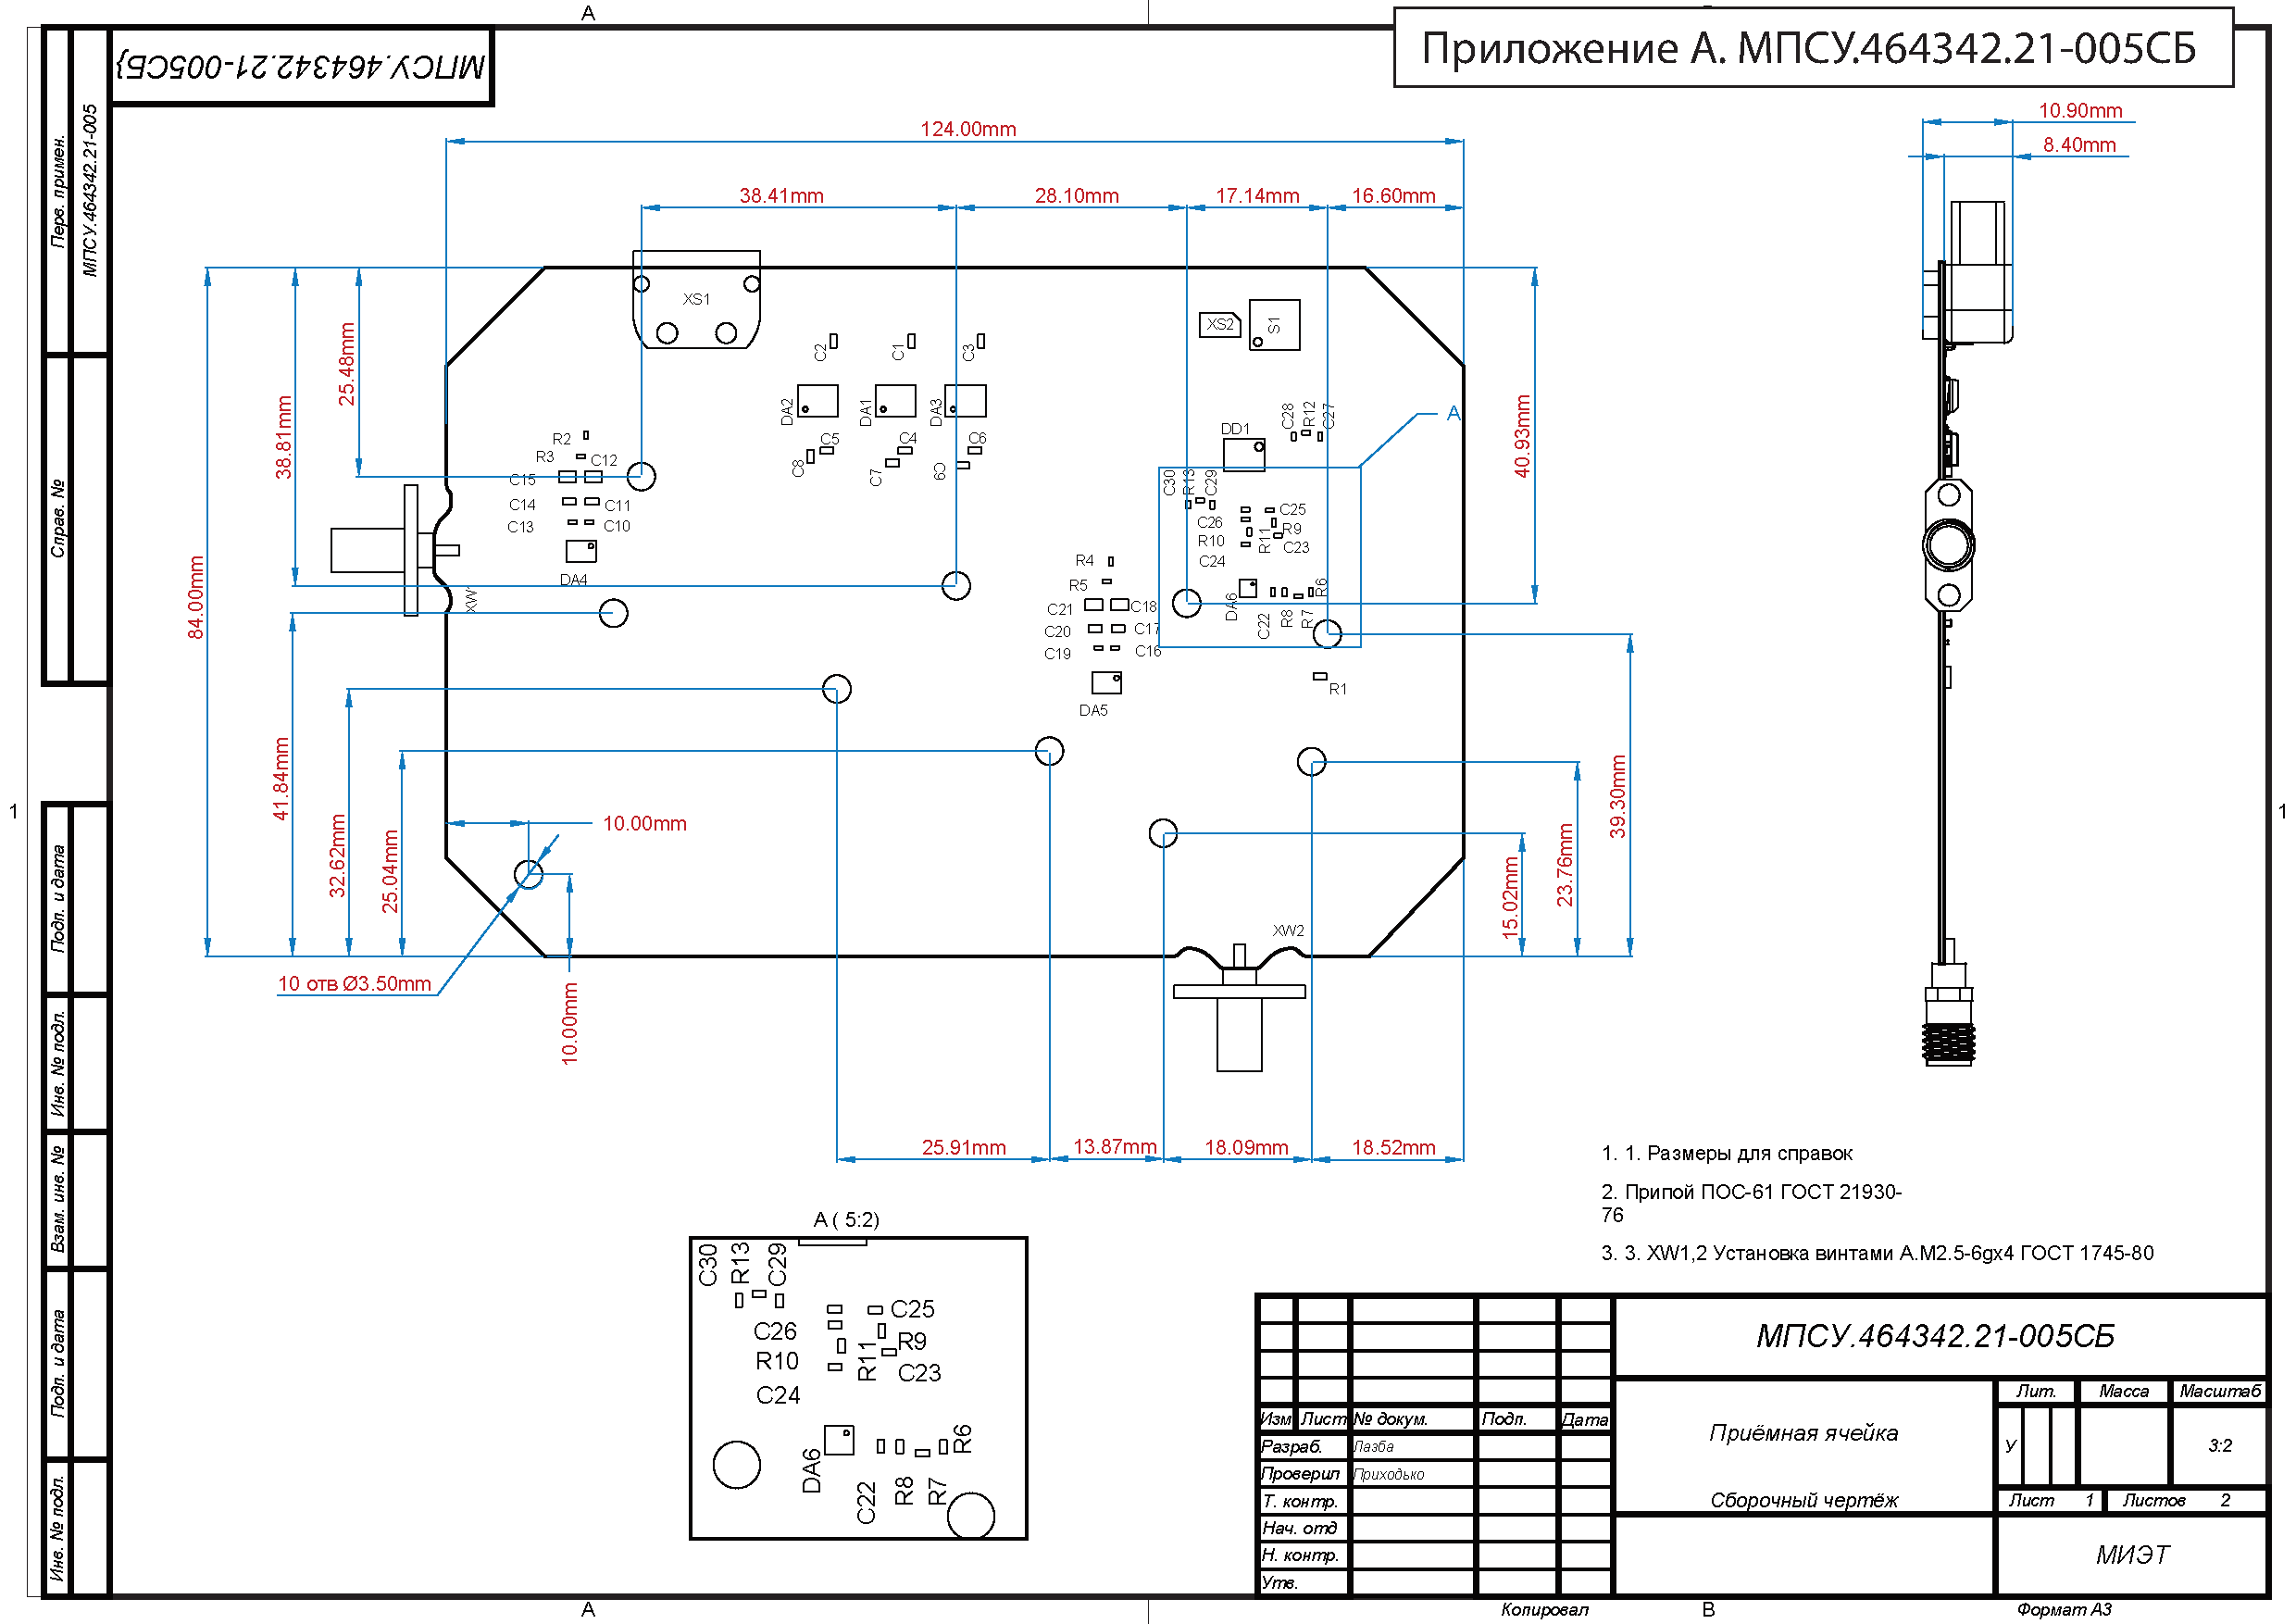
\includegraphics[height=0.33\textheight, page=1]{MPSU.464342.21-005SB.pdf}
	\caption{Сборочный чертёж Лист 1}%
	\label{fig:PU_SB1}
\end{figure}


На второй --- установочные виды компонентов, аннотации для припоя и изометрический вид.
\begin{figure}[H]
	\centering
	\includegraphics[height=0.33\textheight, page=2]{MPSU.464342.21-005SB.pdf}
	\caption{Сборочный чертёж Лист 2}%
	\label{fig:PU_SB2}
\end{figure}

Итоговый файл можно посмотреть в \hyperref[chap:appA]{Приложении А}.
\section[Создание сборочного чертежа на печатную плату]{Создание сборочного чертежа на печатную плату (МПСУ.687254.21-005СБ)}

Выберем шаблон A3. На первый лист добавим главный вид (настроим отображение, проставим размеры) и стек платы. 
\begin{figure}[H]
	\centering
	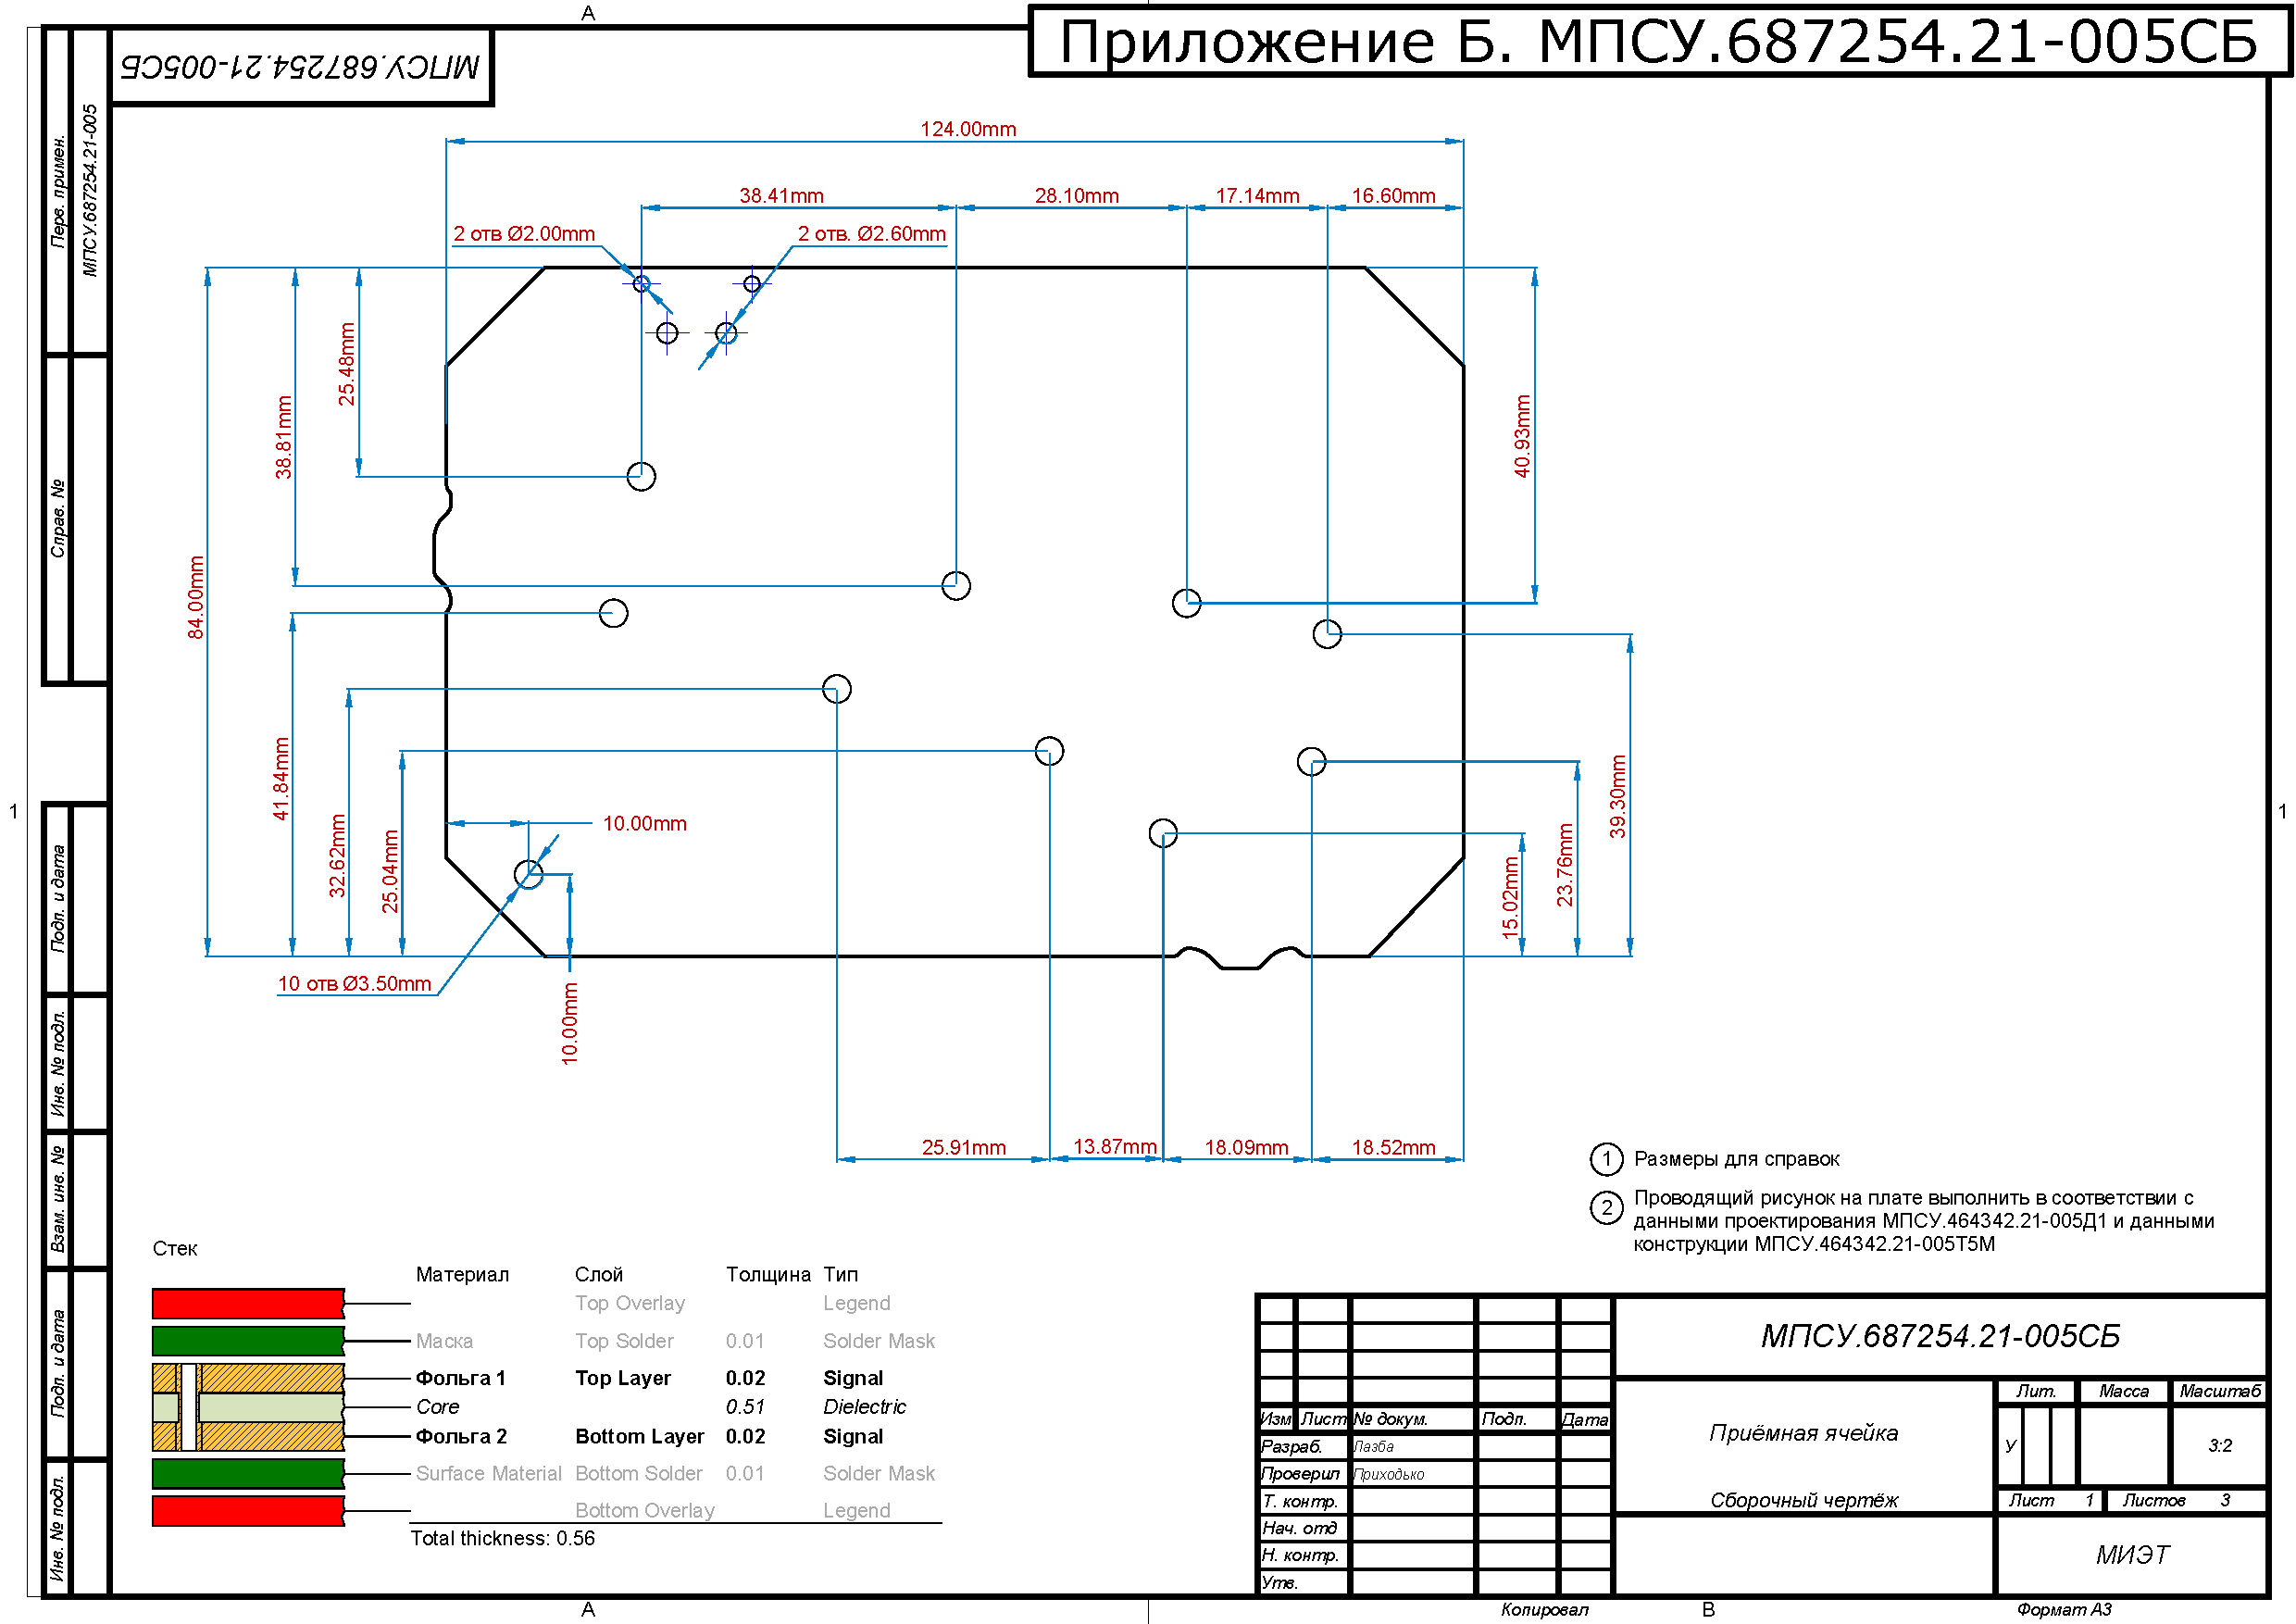
\includegraphics[height=0.32\textheight, page=1]{MPSU.687254.21-005SB.pdf}
	\caption{Сборочный чертёж Лист 1}%
	\label{fig:PCB_SB1}
\end{figure}
На второй - послойное отображение значимых слоёв платы. Для сверки размеров к первому отображению добавим размерную сетку.
\begin{figure}[H]
	\centering
	\includegraphics[height=0.32\textheight, page=2]{MPSU.687254.21-005SB.pdf} 
	\caption{Сборочный чертёж Лист 2}%
	\label{fig:PCB_SB2}
\end{figure}
Итоговый файл можно посмотреть в \hyperref[chap:appB]{Приложении Б}.

\section[Создание данных проектирования на печатную плату]{Создание данных проектирования на печатную плату (МПСУ.687254.21-005Д1)}

Используя встроенное средство CAMtastic создадим GERBER-файлы платы.

\begin{figure}[H]
	\centering
	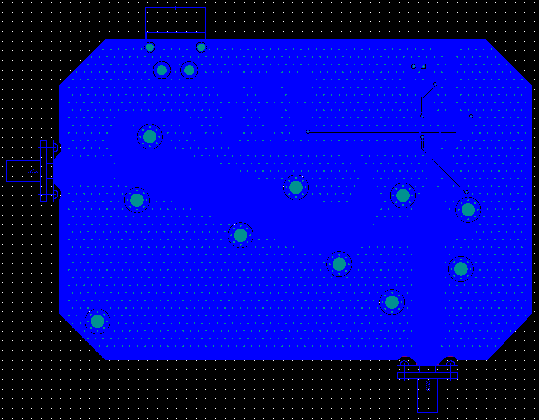
\includegraphics[height=0.3\textheight]{CAMtastic.png}
	\caption{Редактор CAMtastic}%
	\label{fig:CAM}
\end{figure}

Получим следующий список файлов:

\begin{figure}[H]
	\centering
	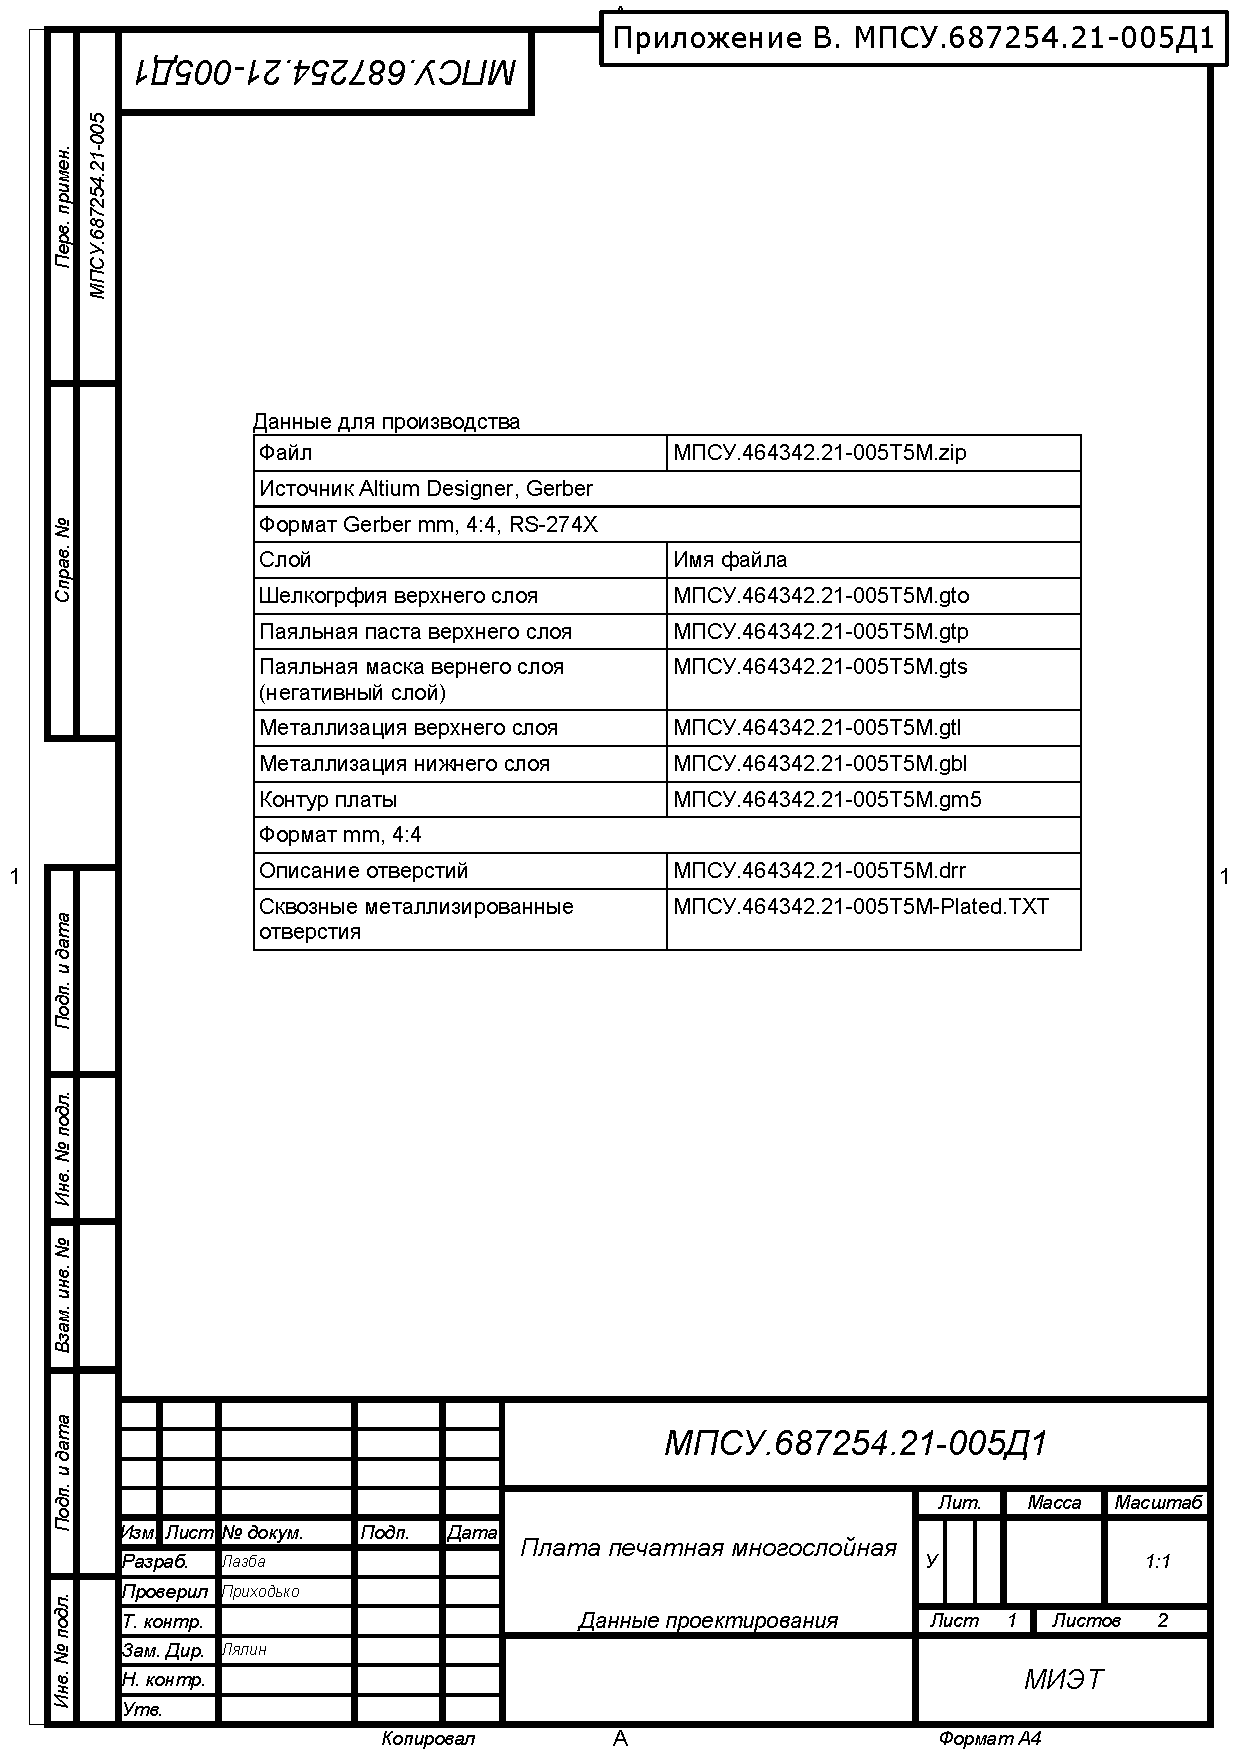
\includegraphics[height=0.3\textheight, page=1, trim={3cm 13cm 2cm 6.5cm}, clip]{MPSU.687254.21-005D1.pdf}
	\caption{Table}%
	\label{fig:PCBData}
\end{figure}

На втором листе отобразим стек платы (его мы уже видели) и таблицу сверловки.

\begin{figure}[H]
	\centering
	\includegraphics[height=0.2\textheight, width=0.9\textwidth, page=2, trim={5cm 12cm 3cm 13.5cm}, clip]{MPSU.687254.21-005D1.pdf}
	\caption{Table}%
	\label{fig:DrillData}
\end{figure}

Итоговый файл можно посмотреть в \hyperref[chap:appC]{Приложении В}.

\section[Экспорт схемы электрической принципиальной]{Экспорт схемы электрической принципиальной (МПСУ.464342.21-005ЭЗ)}

Используем встроенный инструмент SmartPDF. 

\begin{enumerate}
	\item На первом окне надо выбрать, экспортируемся ли 
	весь проект или текущий схематик. Нас интересует весь проект.
	\item В следующем окне надо отметить экспортируемые файлы –  оставляем 
	все, кроме топологии. 
	\item Далее нужно указать, нужно ли экспортировать перечень элементов (по 
	форме BOM). Его мы делаем в отдельном документе ПЭ3, отказываемся.
	\item Далее выбираем создание интерактивного PDF-файла
	\item Указываем чтобы  экспортировалась  схема,  полностью  соответствующая  топологии.
	\item Финализируем PDF без создания файла Output Job.
\end{enumerate}

Итоговый файл можно посмотреть в \hyperref[chap:appD]{Приложении Г}.

\section[Формирование спецификации на печатный узел, 
перечня элементов и ведомости покупных 
изделий]{Формирование спецификации на печатный узел (МПСУ.464342.21-005), перечня элементов (МПСУ.464342.21-005ПЭ3) и ведомости покупных изделий (МПСУ.464342.21-005ВП)}

Эти  документы  можно  сформировать  с  помощью  расширения GOSTBOM, которое входит в российскую поставку Altium Designer.  

Для начала проведём настройки проекта (Reports - GOST BOM - Project Properties) и сортировки элементов (Reports - GOST BOM - Name Mode).

Теперь, по Reports -- GOST BOM -- Make List of Elements создается xls-
файл с перечнем элементов МПСУ.464342.001ПЭ3 и по команде Reports -- GOST BOM -- Make List of Purchased --- МПСУ.464342.001ВП.

Теперь  перейдем  в  редактор  печатных  плат.  Там  по  Reports  --  GOST 
BOM  --  Make  Specification  создадим  спецификацию  на  печатный  узел.  Это 
тоже файл в формате xls.

Видно,  что  в  список  сборочных  единиц  входит  собственно  печатная 
плата  МПСУ.687524.001.  Все  конденсаторы,  резисторы,  индуктивности, 
микросхемы и пр. попали в раздел <<Прочие изделия>>.

Итоговые файлы можно найти в Приложениях \hyperref[chap:appE]{Д}, \hyperref[chap:appE]{Е}, \hyperref[chap:appE]{Ж}.

\section[Формирование спецификации на печатную плату]{Формирование спецификации на печатную плату (МПСУ.687254.21-005)}

Автоматического генератора для спецификации на печатную плату нет, 
возьмем ранее сформированную спецификацию на печатный узел, скопируем 
ее как МПСУ.687254.21-005.xls и отредактируем ее. 

В разделе «Документы» нужно указать сборочный чертеж на печатную 
плату  (МПСУ.687254.21-005СБ),  данные  конструирования (МПСУ.687254.21-005Т5М) и данные проектирования (МПСУ.687254.21-005Д1). В 
раздел «Материалы» внесем информацию об используемых диэлектриках.
 
Также надо не забыть исправить обозначение и наименование изделия. 
Первичное  применение  должно  ссылаться  на  спецификацию  на  печатный 
узел (МПСУ.464214.21-005). 

Итоговый файл можно посмотреть в \hyperref[chap:appH]{Приложении З}.

\section{Формирование спецификации на корпус изделия}

Вообще, это дело должно передаваться в формат настольный режущий плоттер DXF, вырезаться при помощи всяких там станков с ЧПУ и не обременять современного разработчика, но интереса ради я сделал чертёж рамки корпуса. Децимальный номер был выбран 30117.21-005.

\hyperref[chap:appI]{Приложение И}.
